\documentclass{article}

\usepackage{amsmath}
\usepackage{amssymb}
\usepackage{amsfonts}
\usepackage{mathtools}

\usepackage[thmmarks, amsmath]{ntheorem}

\usepackage{fullpage}

\usepackage[inline]{enumitem}


\usepackage[cal=euler]{mathalpha}
%\usepackage{ dsfont }

\usepackage{tikz}
\usepackage{float}

\setlist[enumerate,1]{label=(\alph*)}

\title{Morley Rank as a Game}
\author{Duarte Maia}
%\date{}

\theorembodyfont{\upshape}
\theoremseparator{.}
\newtheorem{theorem}{Theorem}[section]
\newtheorem{prop}[theorem]{Proposition}
\renewtheorem*{prop*}{Proposition}
\newtheorem{lemma}[theorem]{Lemma}
\newtheorem{corollary}[theorem]{Corollary}
\newtheorem{remark}[theorem]{Remark}
\newtheorem{example}[theorem]{Example}
\newtheorem{conjecture}[theorem]{Conjecture}

\theoremsymbol{\ensuremath{\square}}
\newtheorem{prelimdef}[theorem]{Preliminary Definition}
\newtheorem{definition}[theorem]{Definition}

\theoremseparator{:}
\newtheorem{principle}{Principle}

\theoremstyle{nonumberplain}
\theoremsymbol{}
\newtheorem{convention}{Convention}

\theoremheaderfont{\itshape}
\theorembodyfont{\upshape}
\theoremseparator{:}
\theoremsymbol{\ensuremath{\blacksquare}}
\newtheorem{proof}{Proof}
\newtheorem{explanation}{Explanation}
\theoremsymbol{\ensuremath{\text{\textit{(End proof of lemma)}}}}
\newtheorem{lemmaproof}{Proof of Lemma}

\theoremsymbol{\ensuremath{\square}}
\newtheorem{sketch}{Proof Sketch}

\newcommand{\N}{\mathbb{N}}
\newcommand{\Z}{\mathbb{Z}}
\newcommand{\Q}{\mathbb{Q}}
\newcommand{\R}{\mathbb{R}}
\newcommand{\C}{\mathbb{C}}

\newcommand{\Lang}{\mathcal{L}}
\newcommand{\calN}{\mathcal{N}}
\newcommand{\Stone}{\mathrm{S}}
\newcommand{\PStone}{\mathrm{PS}}
\DeclareMathOperator{\Tr}{Tr}
\DeclareMathOperator{\PTr}{PTr}
\DeclareMathOperator{\Th}{Th}
\DeclareMathOperator{\Ext}{Ext}

\DeclarePairedDelimiter{\braket}{\langle}{\rangle}
\DeclarePairedDelimiter{\abs}{\lvert}{\rvert}



\begin{document}
\maketitle

%\tableofcontents

\section{Introduction}

This document provides an alternate way to see and define the notion of Morley rank, as defined in his thesis \cite{morley}. It is written by, and for, someone to whom the relevant definition (Definition 2.2) comes across as random and mysterious. For the sake of brevity, this document does assume some prior knowledge, namely that the reader is familiar with the contents of chapter 1 of \cite{morley}. For the reader who may not be as familiar, or has perhaps forgotten some details, we present very quickly the main required bullet points:
\begin{itemize}
\item We are working with a complete theory $T$ over a countable language $\Lang$, which is assumed to be a relational language,
\item The symbol $\calN(T)$ denotes the collection of submodels of models of $T$,
\item Hypotheses are placed on $T$ such that $\calN(T)$ satisfies several `model-merging' properties. For most practical purposes, these properties may be summarized as follows: Given a collection $\{A_i\}_{i \in I}$ of elements of $\calN(T)$, assuming that these are pairwise compatible (i.e. the relations are well-defined on the intersections $A_i \cap A_j$), the union $\cup_{i \in I} A_i$, possibly with some identifications\footnote{To be more precise about these identifications, it is guaranteed that if $x$ and $y$ are in the same $A_i$ and are distinct there, they will not be identified in the union. The identification phenomenon happens e.g. if the theory says that for some $x \in A_i \cap A_j$ there exists a single $y$ satisfying some property, and both $A_i$ and $A_j$ contain a distinct value for $y$. In this instance, these two values would have to be identified in the union.}, is also in $\calN(T)$.
\end{itemize}

At the time of writing, the author is not entirely sure what happens if these assumptions are foregone, but they are certainly used very frequently in the sequel, and could not be easily discarded. Some attempt to motivate them, or at least interpret their meaning in the framework of this document, may be found below, see Principle \ref{principle:ni} in section \ref{sec:principles}.

\section{The Main Definition and its Consequences}

\subsection{The Motivation}

Suppose that a third party has in their hands a theory $T$ (under the hypotheses of the introduction), a set $A \in \calN(T)$, and a type $p \in \Stone(A)$,\footnote{The Stone space $\Stone(A)$ is the set of types in one variable with parameters in $A$.} and this third party wishes to find out and measure how `slippery' this type is. As a way to measure this, a wager is arranged, between two players. One of which, which we shall imagine as being ourselves, will be dubbed `the Cat', and our goal is to `catch' the type. Our opponent, dubbed `the Mouse', will be controlling the type, and their goal is to run away.

To be more precise, let us elaborate on the rules of the game. At each step, we, the Cat, are allowed to replace $A$ by a bigger set $A' \supseteq A$ in $\calN(T)$. Once we do so, $p \in \Stone(A)$ ceases to be a type, because there are a lot of new sentences which $p$ has to make a decision on. It is the job of the Mouse to make these decisions, and hence decide on an extension $p'$ of $p$ which is a type in $A'$.

Our goal as the Cat is to make clever choices of $A'$, in order to `pin down' the type. The meaning of this expression is not very clear from the outset, and in fact we will see that this ambiguity is the source of a lot of richness in the definition. But a reasonable definition is as thus: We say that a type $p' \in \Stone(A')$ is \emph{pinned down} if, regardless of any future moves $A'' \supseteq A'$ that we as the Cat might make, we can reliably predict what move the Mouse will do. Thus, in some sense, the Mouse has no agency from this point onward, and is immobilized, or stuck.

Let us see some examples to get a feel for this definition.

\begin{example}\label{ex:field}
Let $T$ be (the Morleyization of) the theory of an Algebraically Closed Field of Characteristic Zero. It can be shown that, for $A = \emptyset$, or equivalently $A = \Q$, the types in $\Stone(A)$ come in two kinds: Those which are of the form $p(x) \equiv \braket{P(x) = 0}$, for some irreducible polynomial $P$, and those which are of the form $p(x) \equiv \braket{P(x) \neq 0}_{P \in \Q[x]}$, i.e. `$x$ is transcendent'. Let us give an example of how the game might go in these two cases.
\begin{itemize}
\item Suppose $p(x)$ is the type `$P(x) = 0$', for a fixed irreducible polynomial $P$. Then, we as the Cat might consider adding to $A$ all the roots of $P$; in Field Theory lingo, we would set $A' = \text{the splitting field of $P$}$. After we do so, the Mouse is in trouble. Indeed, $A'$ contains a collection of elements $\lambda_1, \dots, \lambda_n$ such that $P(x)$ may be written (up to a constant term) as
\begin{equation}
P(x) = (x - \lambda_1)\dots(x - \lambda_n),
\end{equation}
and thus, $P(x) = 0$ becomes equivalent to $(x = \lambda_1) \lor \dots \lor (x = \lambda_n)$, and so any extension of $p$ to a type will have to contain one of the formulas $x = \lambda_i$.

We may now say that, no matter the choice that the Mouse makes, they will be trapped. Indeed, regardless of their choice of extension $p' \in \Stone(A')$, their type will now contain a formula $x = \lambda$ for some $\lambda \in A'$, and no matter the choice of $A'' \supseteq A'$ that we make, we will always know that the type $p'$ may only be extended in one way: a formula $\varphi(x)$ is added to the list iff $\lambda$ satisfies it.

This example offers two very strong senses of what it means for the Cat to win the game. One of them is to force the Mouse to extend their type to one containing $x = \lambda$ for some $\lambda \in A'$. Another, weaker in principle if not in fact, is to force the Mouse into a type $p' \in \Stone(A')$ such that, no matter the choice of $A'' \supseteq A'$, there is exactly one extension $p''$ of $p'$ in $\Stone(A'')$. We leave it as an exercise to the reader to verify that these two win conditions are equivalent: if the Cat can win according to one of these conditions, they can win according to the other.

\item Let us now look at the type $p(x)$ of a transcendental element. In this scenario, the game becomes a lot more complicated for the Cat. Indeed, suppose that we were to set, say, $A' = \Q(\pi)$. Then, the Mouse has many choices, as $A'$ includes many transcendental elements $\tau$, and they may, if they so choose, extend the type $p(x)$ to include any such formula $x = \tau$. However, and crucially, they may also choose not to. Indeed, no matter the amount of transcendental elements that the Cat throws into $A'$, the Mouse may simply say `$x$ is neither of those'.

As such, the type $p(x)$ of a transcendental element proves much more slippery that that of an algebraic element: the Cat is \emph{never} able to force the Mouse into picking a concrete element for $x$ to be equal to.

However, it is here that the ambiguity in the definition begins to have its consequences. Indeed, while this is not as clear a win as in the algebraic case, the Cat attempts to argue with the third party that this is in fact a victory for themselves! The reasoning goes as follows:
\begin{quote}
The Mouse isn't stupid. They would never force themselves into the type of a concrete element unless they had to, because they know that this would lose them the game. Therefore, they will always say that they are distinct from, and transcendental over, all the elements that I add into $A'$. As such, I can reliably predict what move the Mouse will make, and so it's pinned down: \emph{I win!}
\end{quote}

The third party is not entirely convinced, and does not respond to this allegation quite yet.
\end{itemize}

Despite the rules-lawyering attempted by the Cat above, it is quite clear that the types in $\Stone(A)$ come in two distinct flavors: the algebraic types, which the Cat is able to pin down in an unambiguous and clear manner, and the transcendental types, for which the situation is more dubious, and hence these are undeniably more slippery.
\end{example}

\begin{example}\label{ex:equiv}
We now consider the theory $T$, (the Morleyization of) the theory of an equivalence relation $E$ with infinitely many classes of infinite size, and suppose for the sake of concreteness that $A$ is a countable model of $T$, though the following analysis holds for any $A \in \calN(T)$. We visualize $A$ and $\Stone(A)$ via the following diagram.
\begin{figure}[H]
\centering
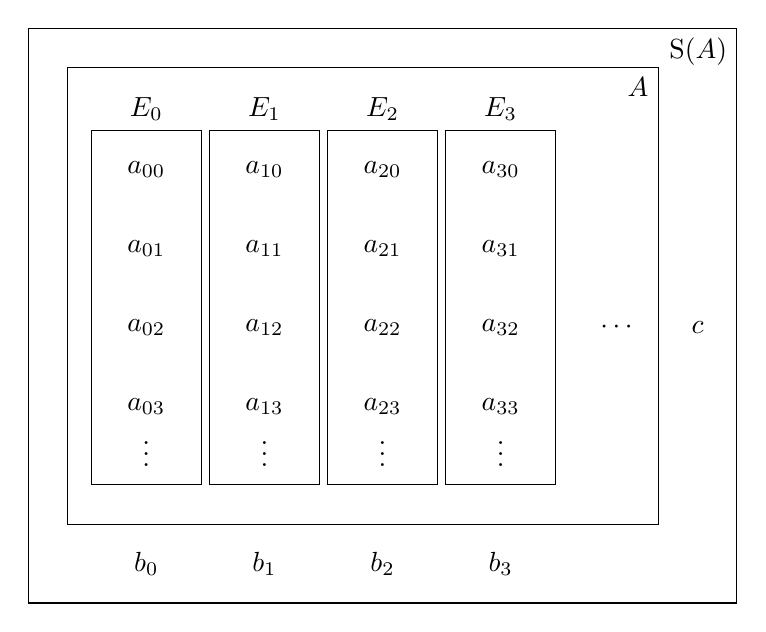
\begin{tikzpicture}
\foreach \i in {0,...,3} {
\foreach \j in {0,...,3} {
\node at (1.5*\i,-\j) {$a_{\i\j}$};
}
\node at (1.5*\i, -3.5) {$\vdots$};
\draw (1.5*\i, 0) + (-0.7, 0.5) rectangle +(0.7,-4);
\node[above] at (1.5*\i,0.5) {$E_\i$};
}
\node at (1.5*3 + 1.5, -2) {$\cdots$};

\draw (-1, 1.3) rectangle (6.5,-4.5);
\node[below left] at (6.5,1.3) {$A$};

\foreach \i in {0,...,3} {
\node at (1.5*\i, -5) {$b_\i$};
}

\node at (1.5*4 + 1, -2) {$c$};

\draw (-1.5, -5.5) rectangle (7.5,1.8) node[below left] {$\Stone(A)$};
\end{tikzpicture}
\caption{A visual representation of $A$ and $\Stone(A)$. The $a_{ij}$ are the elements of $A$, with $a_{ij}$ being in the equivalence class $E_i$. The type $b_i$ is that of an element in the $i$-th equivalence class, but distinct from all $a_{ij}, j \in \N$. The type $c$ is that of an element which is not equivalent to any $a_{ij}$.}
\end{figure}

Now, let us investigate how the game plays on this new board.
\begin{itemize}
\item If $p$ is one of the $a_{ij}$, the Mouse has lost the game from the very beginning.

\item If $p$ is one of the $b_i$, we are in a similar situation as the transcendent elements from example \ref{ex:field}. No matter what sort of elements the Cat adds to $A$, the Mouse can always avoid making their type the type of any particular element. However, also as in example \ref{ex:field}, the Cat tries to argue that the Mouse is pinned down, because unless the Mouse plays to their own detriment, the Cat can always predict the Mouse's moves.

\item Finally, if $p = c$, the Mouse now has a certain amount of freedom. Indeed, when the Cat adds a new element $a_\omega$, the Mouse may (without committing to any particular element) choose whether to complete the type by adding the formula $E(x,a_\omega)$ or its negation, and so the Cat cannot argue as immediately that this also counts as a win condition for themselves. But they try anyway.
\begin{quote}
As we've seen before, any of the types $b_i$ are actually a loss for the Mouse, right? Because if the Mouse is not playing to lose, they never actually have a choice about how to increase the type when I add a new element. Now, if you'll look at the type $c$, when I add a new element $a_\omega$, the Mouse is never going to add the formula $E(x,a_\omega)$... If they did, they would now be in the condition of a type $b_\omega$, of an element which is in a known equivalence class despite not being any of the elements on the game board, and this is, as I've argued, a losing condition! Therefore, I can be safe in knowing that the Mouse will always add the formula $\neg E(x,a_\omega)$...
\end{quote}
\end{itemize}
\end{example}

Facing this situation, the rules-arbiter third party finally responds to the Cat's allegations. Assuming the scenario of example \ref{ex:equiv} for the sake of concreteness, the ruling goes as follows.
\begin{quote}
It is clear that the types of $\Stone(A)$ come in three different categories of `slipperiness'. Those which correspond to elements of $A$ are an unambiguous loss, and to those, I assign a score of $0$. To the types $b_i$, which are a loss only in a more dubious sense, I assign a score of $1$, indicating that they are more-or-less a loss for the Mouse, but not as much as the $a_{ij}$. Finally, to the type $c$, I assign a score of $2$, because any attempt at arguing that $c$ is a loss is predicated on acceptance that the $b_i$ are a loss, thereby making $c$ a loss which is twice as dubious as that of $b_i$.

More generally, I will assign to every type in $\Stone(A)$ (now in an arbitrary theory $T$) a score $\alpha$, detailing how many distinct times the Cat must argue over rules with me before being able to declare the type a win for themselves.
\end{quote}

This ruling mostly clears up the ambiguities in the original rules of the game. We summarize it via the following definition. In it, $\Tr_0^\alpha(A)$ represents the set of elements for which the Cat wins the game, with best possible score equal to $\alpha$.
\begin{definition}\label{def:tr01}
Let $T$ be a theory in the hypotheses of the introduction, and $A \in \calN(T)$. We inductively define the sets $\Tr_0^\alpha(A) \subseteq \Stone(A)$, for $\alpha$ an ordinal number, via the following procedure. Assuming $\Tr_0^\beta(B)$ has been defined for all $\beta < \alpha$ and $B \in \calN(T)$, we say that $p \in \Stone(A)$ is in $\Tr_0^\alpha(A)$ if:
\begin{itemize}
\item $p$ is not in $\Tr_0^\beta(A)$ for any $\beta < \alpha$,
\item There is some $A' \supseteq A$ such that any extension of $p$ to a type $p' \in \Stone(A')$ is $\alpha$-pinned down, in the following sense:
\item We say $p' \in \Stone(A')$ is \emph{weakly $\alpha$-pinned down} if, for every $A'' \supseteq A'$, there is at most one extension of $p'$ to a type $p'' \in \Stone(A'')$ that is not in $\cup_{\beta < \alpha} \Tr_0^\beta(A'')$.
\end{itemize}
\end{definition}

Unfortunately, appealing though the above definition may be based on this game-theoretic interpretation, it may or may not coincide with Morley's definition; see conjecture \ref{conj:lemma} below. In essence, our definition of a type being pinned down is too weak: for technical reasons we desire that, if a type $p$ is pinned down, it is so because of a finite amount of information contained in $p$; our definition does not \textit{a priori} guarantee that this is the case.

In an effort to preserve the fiction developed above, we may imagine the rules being adapted as follows: Annoyed at the Cat's persistence in trying to eke out a win for themselves, the third party adapts the rules as we've discussed, with one caveat: It is the Cat's responsibility to provide proof that the Mouse is indeed pinned down, by supplying some finite amount of information in the Mouse's position that makes it untenable.

\begin{definition}\label{def:tr1}
Let $T$ be a theory in the hypotheses of the introduction, and $A \in \calN(T)$. We inductively define the sets $\Tr^\alpha(A) \subseteq \Stone(A)$, for $\alpha$ an ordinal number, via the following procedure. Assuming $\Tr^\beta(B)$ has been defined for all $\beta < \alpha$ and $B \in \calN(T)$, we say that $p \in \Stone(A)$ is in $\Tr^\alpha(A)$ if:
\begin{itemize}
\item $p$ is not in $\Tr^\beta(A)$ for any $\beta < \alpha$,
\item There is some $A' \supseteq A$ such that any extension of $p$ to a type $p' \in \Stone(A')$ is $\alpha$-pinned down, in the following sense:
\item We say $p' \in \Stone(A')$ is \emph{(strongly) $\alpha$-pinned down} if there is some formula $\varphi \in p'$ such that, for every $A'' \supseteq A'$, there is at most one type $p'' \in \Stone(A'')$ containing $\varphi$ that is not in $\cup_{\beta < \alpha} \Tr^\beta(A'')$.
\end{itemize}
\end{definition}

One may wonder how much this requirement affects the Cat's performance. We begin with a proposition which is positive in the Cat's direction

\begin{prop}
A type $p' \in S(A')$ is weakly $0$-pinned down iff it is strongly $0$-pinned down.
\end{prop}

\begin{proof}
In the remainder of this proof, we will omit the numeral $0$, and write (weakly) pinned down for (weakly) $0$-pinned down.

It is evident that if a type $p'$ is strongly pinned down, then it is weakly pinned down. Thus, we turn to showing the converse.

If $p'$ is weakly pinned down, then in particular any model of $T$ (containing $A'$) can realize $p'$ at most once. Thus, the following theory (on the language of $A'$, plus two constant symbols $c$ and $d$) is inconsistent:
\begin{equation}
\text{The theory of $A'$} + p'(c) + p'(d) + (c \neq d).
\end{equation}

By compactness, one obtains a formula $\varphi \in p'$ such that, in fact, the theory of $A'$ plus $\varphi(c) \land \varphi(d) \land (c \neq d)$ is inconsistent. Equivalently,
\begin{equation}
\text{The theory of $A'$} \vdash \forall_x \forall_y (\varphi(x) \land \varphi(y) \rightarrow x = y).
\end{equation}

We claim that the formula $\varphi$ isolates $p'$ in $\Stone(A')$. Indeed, suppose that there was some other type $q \in \Stone(A')$ containing $\varphi$. Then, there is a model $M_{p'} \supseteq A'$ realizing $p'$, and a model $M_q \supseteq A'$ realizing $q$. By the model gluing properties discussed in the introduction, there is a model $M$ of the theory of $A'$ containing a copy of both of these models, and thus containing some element $x \in M$ realizing $p'$, and another $y \in M$ realizing $q$. These must be distinct, i.e. $x \neq y$, because they have distinct types. But of course, this is a contradiction, which completes the proof.
\end{proof}

\begin{corollary}
Given a theory $T$ and some $A \in \calN(T)$, we have $\Tr_0^0(A) = \Tr^0(A)$.
\end{corollary}

The author does not at this moment know whether this results holds at higher ranks.

\begin{conjecture}\label{conj:lemma}
A type $p \in \calN(A)$ is weakly $\alpha$-pinned down (with respect to $\Tr^\alpha(A)$) iff it is strongly $\alpha$-pinned down. This implies that $\Tr_0^\alpha(A) = \Tr^\alpha(A)$ for all ordinals $\alpha$.
\end{conjecture}

\subsection{Some Principles of Reasoning}\label{sec:principles}

Before presenting a rigorous study of definition \ref{def:tr1}, it is useful to present some principles which the author finds helpful in guiding his thinking. These principles refer to the game-theoretic view of definition \ref{def:tr1}, and the idea is that they clarify ideas and arguments which will be common in the sequel. They may be turned into rigorously written propositions, and indeed will be, but the goal is to present them in an intuitive manner as not to lose sight of the forest for the trees.

Before these intuitive principles, we present a useful lemma, whose truthfulness is obvious from the definitions involved.

\begin{lemma}\label{lemma:pdmono}
Let $p \in \Stone(A)$ be $\alpha$-pinned down. Then, it is also $\beta$-pinned down for all $\beta \geq \alpha$. Moreover, if $A' \supseteq A$, any extension of $p$ to a type $p' \in \Stone(A')$ is also $\alpha$-pinned down.
\end{lemma}

In the following, we refer to the notion of `slipperiness' of a type which definition \ref{def:tr1} attempts to embody.

\begin{principle}[Monotony]\label{principle:mono}
Adding elements to $A \in \calN(T)$ will never increase a type's slipperiness, but may decrease it. Conversely, removing elements from $A$ will never decrease a type's slipperiness, but may increase it. 
\end{principle}

\begin{explanation}
The Cat's goal is to add more elements to $A$, ending with $A'$ say, in order to force the Mouse to extend the type at hand, say $p$, to one which is pinned down to some rank $\alpha$. If $A$ is replaced by $A^* \supseteq A$, the type $p \in \Stone(A)$ may be extended to a type $p^* \in \Stone(A^*)$ in multiple ways. However, the most slippery way to do so is at most $\alpha$-slippery and here is why: Let $A' \supseteq A$ be a model such that any extension of $p$ to $\Stone(A')$ is $\alpha$-pinned down. Then, by the model-gluing properties discussed in the introduction, there is a model $A^{**}$ which contains a copy of $A'$ and $A^*$. Since it contains $A'$, any extension of $p$ to a type in $A^{**}$ is $\alpha$-pinned down, and it is not hard to see that any extension of $p^*$ To a type in $A^{**}$ is also an extension of $p$. Hence, any extension of $p^*$ to a type in $A^{**}$ is $\alpha$-pinned down, whence $p^*$ is at most $\alpha$-slippery.
\end{explanation}

\begin{remark}
Above, we said that the most slippery way to extend $p$ to $p^*$ is at most $\alpha$-slippery; It is not obvious that there is an $\alpha$-slippery way. This uses in an essential way the finite information principle, principle \ref{principle:fininfo} below, and is investigated rigorously in lemma \ref{lemma:ext} below.
\end{remark}

Implicit in the explanation of principle \ref{principle:mono} is an invocation of the following principle, which embodies the necessity of the model-gluing properties.

\begin{principle}[Non-Interference]\label{principle:ni}
Increasing $A$ is never prejudicial for the Cat. More generally, the Cat's moves never interfere with one another.
\end{principle}

\begin{explanation}
If it is beneficial for the Cat to increase $A$ to a bigger set $A'$, increasing it first to some other $A^*$ is not a problem, because by the model-gluing properties one can always find some $A^{**}$ containing a copy of both.
\end{explanation}

The last principle is self-explanatory, and will be the first one to be made rigorous, in proposition \ref{prop:open}.

\begin{principle}[Finite Information]\label{principle:fininfo}
Every victory by the Cat is predicated on finite amounts of information, due to the third party's requirement that any claim that a type is pinned down must be justified by a finite amount of information present in the type.
\end{principle}

\subsection{Consequences}

We now develop the definition of $\Tr^\alpha(A)$, establishing a collection of properties in line with the ones established in \cite{morley}, with this alternate definition in focus. We will make some attempt to interpret these properties in game-theoretic terms, pointing out how they relate to the principles laid out in the previous section.

Before doing so, we define some notation.

\begin{definition}
Given a theory $T$, $A \in \calN(T)$, and an ordinal $\alpha$, we set $\Stone^\alpha(A) := \Stone(A) \setminus \bigcup_{\beta < \alpha} \Tr^\beta(A)$. We also define $\Tr^{<\alpha}(A) := \bigcup_{\beta < \alpha} \Tr^\alpha(A)$, and $\Tr^{\leq\alpha}(A) := \Tr^{<(\alpha+1)}(A)$.
\end{definition}

\begin{definition}
If $i \colon A \to A'$ is the inclusion map $A \subseteq A'$ (or, more generally, a monomorphism) we define $i^* \colon \Stone(A') \to \Stone(A)$ to be the `forgetful map', which given a type $p' \in \Stone(A')$ forgets all the information it has about elements of $A' \setminus A$.
\end{definition}

\begin{definition}
Let $A \subseteq A'$ be two elements of $\calN(T)$, and let $p \in \Stone(A)$. We define $\Ext^0(p, A')$, or simply $\Ext(p,A')$, to be the collection of extensions of $p$ to types in $A'$. More generally, if $\alpha$ is an ordinal, we set $\Ext^\alpha(p, A')$ to be the set of such extensions which are in $\Stone^\alpha(A')$. Symbolically, if $i$ is the inclusion map,
\begin{equation}
\Ext^\alpha(p,A') := (i^*)^{-1}(p) \cap \Stone^\alpha(A').
\end{equation}
\end{definition}

Morley also establishes a topological structure on $\Stone(A)$. A first draft of this document attempted to avoid the topological nomenclature as much as possible, but this quickly became more burdensome than it was worth. Thus, we will make use of this topological structure in our proofs. However, we will eunciate our propositions in a way that does not require knowledge of this topology to interpret.

In the sequel, we assume fixed a theory $T$ in the conditions of the introduction.

The first proposition is a strong embodiment of principle \ref{principle:fininfo}: Not only does it say that the slipperiness of a type is encoded in a single one of its formulas, but it also says that a type $p$ which is not a win for the Mouse may be identified unequivocally by: The unique type at so-and-so level of slipperiness containing such-and-such formula.

\begin{prop}\label{prop:open}
Given $A \in \calN(T)$ and an ordinal $\alpha$, the set $\Tr^{<\alpha}(A)$ is open, in the following sense: Given $p \in \Tr^{<\alpha}(A)$, there is some $\varphi \in p$ such that any type containing $\varphi$ is in $\Tr^{<\alpha}(A)$. More strongly, given $p \in \Tr^\alpha(A)$, $\varphi \in p$ may be chosen such that all types containing $\varphi$, with the exception of $p$, are in $\Tr^{<\alpha}(A)$.

As a consequence, the set $\Stone^\alpha(A)$ is compact, in the following sense: Given a collection $\{\varphi_i\}_{i \in I}$ of formulas such that any $p \in \Stone^\alpha(A)$ contains some $\varphi_i$, there is a finite subset $\{\varphi_i\}_{i \in I_0}$ with this property.
\end{prop}

\begin{proof}
We will prove only the strong `openness' assertion. Compactness follows from this and the compactness of $\Stone(A)$, which in turn follows from the compactness of first order logic.

This proof will be performed by strong induction on $\alpha$. That is, given a fixed $\alpha$, we assume that the strong openness property has been proven true for all $\beta < \alpha$, and for all $A \in \calN(T)$. This in particular implies that $\Tr^{<\alpha}(A)$ is open, and so that $\Stone^\alpha(A)$ is compact.

Let $p \in \Tr^\alpha(A)$. Then, there is a model $A' \supseteq A$ such that all elements of $\Ext(p, A')$ are $\alpha$-pinned down. The game plan is as follows: We will find a formula $\psi$ (in $A'$) which covers $\Ext(p,A')$, without leaving $\Ext(p,A') \cup \Tr^{<\alpha}(A')$. This formula may use language from $A'$, so we find a formula $\varphi$ in $p$ which implies $\psi$. This is the formula that will isolate $p$ in $\Stone^\alpha(A)$.

We begin by finding $\psi$. First, by the induction hypothesis, $\Tr^{<\alpha}(A')$ is open. Moreover, applying the definition of $p' \in \Ext(p,A')$ being $\alpha$-pinned down to $A'' = A'$, we obtain that for every such $p'$ there is a neighborhood of $p'$ contained in $\{p'\} \cup \Tr^{<\alpha}(A')$. As a consequence, we conclude that $\Ext(p,A') \cup \Tr^{<\alpha}(A')$ is open in $\Stone(A')$, and since $\Ext(p,A')$ is compact,\footnote{This is because $\Ext(p,A')$ is a closed subset of the compact space $\Stone(A')$. Closedness of $\Ext(p,A')$ may be shown using the continuity of $i^* \colon \Stone(A') \to \Stone(A)$, as Morley does, but here is a more direct proof: By definition, if $q \not\in \Ext(p,A')$, there is some formula $\eta \in p$ whose negation is in $q$. Thus, $\neg\eta$ induces a neighborhood of $q$ which does not intersect $\Ext(p,A')$.} there is a basic open $U_\psi$, such that
\begin{equation}
\Ext(p,A') \subseteq U_\psi \subseteq \Ext(p,A') \cup \Tr^{<\alpha}(A').
\end{equation}

Let us first look at the inclusion $\Ext(p,A') \subseteq U_\psi$. This means that any extension of $p$ to a type in $\Stone(A')$ will contain $\psi$, and by compactness of first-order logic it follows that there is some $\varphi \in p$ such that $A' \vDash \varphi(x) \rightarrow \psi(x)$. We claim that this is the formula we desire, which will isolate $p$ from the rest of $\Stone^\alpha(A)$.

To prove this claim, let $q$ be a type in $\Stone^\alpha(A)$ containing $\varphi$. Then, any extension of $q$ to a type in $\Stone(A')$ will be in $U_\varphi$, and hence in $\Ext(p,A') \cup \Tr^{<\alpha}(A')$. We now require the following lemma.

\begin{lemma}\label{lemma:ext}
Given $A, A' \in \calN(T)$ such that $A \subseteq A'$, an ordinal $\alpha$, and a type $q \in \Stone^\alpha(A)$, there is an extension of $q$ to a type $q' \in \Stone^\alpha(A')$. In other words, if $q \in \Stone^\alpha(A)$ then $\Ext^\alpha(q,A') \neq \emptyset$.
\end{lemma}

\begin{remark}
See also principle \ref{principle:mono} above.
\end{remark}

\begin{lemmaproof}
Suppose that all extensions of $q$ to types in $\Stone(A')$ are in $\Tr^{<\alpha}(A')$. Then, by compactness of $\Ext(q,A')$ and openness of $\Tr^{\leq \beta}(A')$ for $\beta < \alpha$ (by the induction hypothesis), we get that all extensions of $q$ to types in $\Stone(A')$ are in fact contained in some fixed $\Tr^{\leq \beta}$, with $\beta < \alpha$. We show that $q \in \Tr^{\leq \beta}(A)$, a contradiction.

Suppose that $q \not\in \Tr^{<\beta}(A)$. Then, we will show that $q \in \Tr^\beta(A)$. To do this, we note that for every $q' \in \Ext(q,A')$ there is a model $A^*_{q'}$ extending $A'$ such that every element of $\Ext(q',A^*_{q'})$ is $\beta$-pinned down.\footnote{This uses the fact that if a type is $\gamma$-pinned down for some $\gamma \leq \beta$, then it is also $\beta$-pinned down; see lemma \ref{lemma:pdmono}.} By the model-gluing properties in the introduction (see also principle \ref{principle:ni}), define $A^*$ as a model containing a copy of every $A^*_{q'}$. It is easy to verify then by definition that every extension of $q$ to a type in $\Stone(A^*)$ is $\beta$-pinned down. As such, $q$ is in $\Tr^\beta(A)$, as desired.
\end{lemmaproof}

Continuing the proof, by the lemma we have an extension of $q$ to a type $q' \in \Stone^\alpha(A')$. But since $q$ contains $\varphi$, this implies that $q' \in \Ext(p,A')$, and hence $q = p$, as desired.
\end{proof}

\begin{remark}
Proposition \ref{prop:open} corresponds directly to Theorem 2.3 (a) in \cite{morley}, and lemma \ref{lemma:ext} is reminiscent of Theorem 2.3 (b). For completeness, we make the latter connection explicit.
\end{remark}

\begin{prop}\label{prop:istone}
Let $A, A' \in \calN(T)$ such that $A \subseteq A'$, with $i$ the inclusion map. Then we have \begin{enumerate*} \item\label{item:1} $i^*(\Stone^\alpha(A')) = \Stone^\alpha(A)$, and \item\label{item:2} an element $p \in \Stone^\alpha(A)$ is in $\Tr^\alpha(A)$ iff all of its extensions to types in $\Stone^\alpha(A')$ are in $\Tr^\alpha(A')$.\end{enumerate*}
\end{prop}

\begin{proof}
Lemma \ref{lemma:ext} is half of the statement of \ref{item:1}, as it proves that $i^*(\Stone^\alpha(A')) \supseteq \Stone^\alpha(A)$. The other inclusion is clear: If a type $p' \in \Stone^\alpha(A')$ is \emph{not} a losing position for the mouse (with score less than $\alpha$), then making the model any smaller will not make it so, as the Mouse benefits from having less expressive power in the language (principle \ref{principle:mono}). More formally, if $i^*(p')$ was in a $\beta$-losing position for the Mouse, then the move $A^*$ that the Cat can make from $A$ could also have been made starting from $A'$ (using the model-gluing properties to create a model that contains a copy of both $A'$ and $A^*$).

Let us now prove \ref{item:2}. The implication $(\rightarrow)$ is interpreted as: When the Cat makes a move, Mouse can never change to a less-losing position. Indeed, if a type $p \in \Stone^\alpha(A)$ cannot be extended to a type $p' \in \Stone^\alpha(A^*)$ without being pinned down, then an extension of $p$ to a type $p'$ in $\Stone^\alpha(A')$ can also not be extended to a type in $(A^* \cup A')/\sim$ without being pinned down (see lemma \ref{lemma:pdmono}). On the other hand, $(\leftarrow)$ if $p \in \Stone^\alpha(A)$ but all of its extensions $p'$ in $\Stone(A')$ are in an $\alpha$-losing position for the Mouse, using an argument similar to the one used in lemma \ref{lemma:ext} to create an extension $A^*$ of $A'$ such that all extensions of all $p'$ are $\alpha$-pinned down, this same extension $A^*$ may be used as the Cat's move to show that $p \in \Stone^\alpha(A)$ is an $\alpha$-losing position for the Mouse.
\end{proof}

The above proof yields much more than the proposition it sought to establish. We provide some other consequences.

The following proposition is Corollary 2.4 in \cite{morley}.

\begin{prop}\label{prop:f}
If $p \in \Tr^\alpha(A)$ then there is a finite $F \subseteq A$ (with inclusion $i$) such that $i^*(p) \in \Tr^\alpha(F)$.
\end{prop}

\begin{proof}
In the proof of proposition \ref{prop:open} we found a single formula $\varphi \in p$ such that any type in $\Stone(A')$ containing $\varphi$ would be $\alpha$-pinned down. As such, if $F$ is any subset of $A$ containing all the constant symbols used in $\varphi$, $i^*(p)$ will be a lost position to the Mouse, with score at most equal to $\alpha$, since the Cat can make the move $A' \supseteq F$. This leaves open the possibility that $i^*(p)$ would lose with a worse score for the Mouse, but as we have already discussed, by principle \ref{principle:mono} decreasing the expressive power of the language is advantageous for the Mouse.
\end{proof}

\begin{lemma}\label{lemma:deg}
If $p \in \Tr^\alpha(A)$ and $A' \supseteq A$, $\Ext^\alpha(p, A')$ is finite.
\end{lemma}

\begin{proof}
The set $\Ext(p,A')$ is compact, and admits the following covering by opens. One of the opens is given by $\Tr^{<\alpha}(A')$. Then, for each $p' \in \Ext^\alpha(p,A')$, we build a neighborhood of $p'$ as given by proposition \ref{prop:open}, which is contained in $\{p'\} \cup \Tr^{<\alpha}(A')$. (This requires verifying that $p' \in \Tr^\alpha(A')$; see principle \ref{principle:mono}.)

By compactness, this cover admits a finite subcover of $\Ext(p,A')$. However, the only open set which might possibly be removed is $\Tr^{<\alpha}(A')$. Thus, the cover must have been finite to begin with, and there must be finitely many $p' \in \Ext^\alpha(p,A')$.
\end{proof}

We have the following extension of proposition \ref{prop:f}, which can be interpreted game-theoretically as: The Cat loses nothing by restricting themselves to finite moves.

\begin{prop}
Let $p \in \Tr^\alpha(A)$. Then, there is a \emph{finite} extension of $A$, say $A'_0 \supseteq^{\text{fin}} A$, such that every extension of $p$ to a type in $\Stone(A'_0)$ is $\alpha$-pinned down.
\end{prop}

\begin{proof}
Let $A' \supseteq A$ be a winning move for the Cat, and let $\psi_1, \dots, \psi_n$ be the formulas ensuring that the elements of $\Ext^\alpha(p,A')$ are $\alpha$-pinned down. There are finitely many by lemma \ref{lemma:deg}, and so we define $A'_0$ as the set $A$, together with the elements of $A'$ taking part in the formulas $\psi_i$. Then, it can be seen that $p$ extends to an $\alpha$-slippery type in $A'_0$ in exactly $n$ ways, exactly one for each $\psi_i$ (and no more by lemma \ref{lemma:ext}), and using model-gluing properties one obtains that each of these types is itself $\alpha$-pinned down. Hence, $A'_0$ is a winning move for the Cat.
\end{proof}

We now define the notion of degree. Parts \ref{item:11} and \ref{item:12} of the following proposition correspond to Theorem 2.5 in \cite{morley}. Part \ref{item:13} is our own addition.

\begin{prop}
\begin{enumerate}
\item\label{item:11} If $p \in \Tr^\alpha(A)$ there is an integer $n$ such that, for every $A' \supseteq A$, $\Ext^\alpha(p,A')$ has at most $n$ elements. The least such $n$, or equivalently the maximum possible number of elements, is referred to as the \emph{degree of $p$}.

\item\label{item:12} If $p \in \Tr^\alpha(A)$ and $A' \supseteq A$, then
\begin{equation}\label{eq:deg}
\deg(p) = \sum_{q \in \Ext^\alpha(p,A')} \deg(q).
\end{equation}

\item\label{item:13} If $p \in \Tr^\alpha(A)$ and $A' \supseteq A$ is a winning move for the Cat (i.e. every $p' \in \Ext(p,A')$ is $\alpha$-pinned down), the degree of $p$ is the number of elements of $\Ext^\alpha(p,A')$.
\end{enumerate}
\end{prop}

\begin{proof}
Parts \ref{item:11} and \ref{item:12} may be proved in a way similar to \cite{morley}, and \ref{item:13} is a direct consequence of \ref{item:12}. However, we will instead prove \ref{item:13} directly, and from it conclude the other two.

First, we note that if $A'$ and $A^*$ are both winning moves for the Cat, the type $p$ has the same number of extensions to $\alpha$-slippery types in each. To prove this, we build a one-to-one correspondence between them. Indeed, let $A^{**}$ be a model containing a copy of both $A'$ and $A^*$. Then, since all extensions of $p$ to types in either $A'$ or $A^*$ are $\alpha$-pinned down, each type in e.g. $\Ext^\alpha(p, A')$ has at most one extension to $\Stone^\alpha(A^{**})$, and likewise for $A^*$; by lemma \ref{lemma:ext} there is in fact \emph{exactly} one extension. Since we have
\begin{equation}
\bigcup_{p' \in \Ext(p,A')} \Ext(p', A^{**}) = \Ext(p, A^{**})
\end{equation}
we conclude that the map $(p' \mapsto \text{The unique element of $\Ext(p', A^{**})$})$ furnishes a one-to-one correspondence between $\Ext^\alpha(p, A')$ and $\Ext^\alpha(p,A^{**})$. In a similar fashion, we have a one-to-one correspondence between the latter and the extensions of $p$ in $\Stone^\alpha(A^*)$, and the proof of \ref{item:13} is complete.\footnote{Technically, we have not proven \ref{item:13}, as we have not defined the degree as in the statement. What we have done is shown that the number of elements in $\Ext^\alpha(p,A')$ is independent of $A'$ (so long as it is a winning move for the Cat), and we implicitly define this number as the degree of $p$.}

We now sketch the proofs of \ref{item:11} and \ref{item:12}. For \ref{item:11}, let $A'$ be arbitrary, and let $A^*$ be an extension of $A'$ which is a winning move for the Cat starting at $p \in \Tr^\alpha(A)$ (this uses principle \ref{principle:ni}). Now, by lemma \ref{lemma:ext}, every extension of $p$ to a type in $\Stone^\alpha(A')$ has in turn at least one extension to a type in $\Stone^\alpha(A^*)$, and all of these are distinct. Thus,
\begin{equation}
\#\Ext^\alpha(p,A') \leq \#\Ext(p, A^*) = \deg(p).
\end{equation}

Thus, $p$ can be extended to at most $n = \deg(p)$ distinct $\alpha$-slippery types in $A'$, no matter the choice of $A'$, and of course this upper bound is attained if $A'$ is a winning move for the Cat.

This proof may be adapted without much effort into a proof of \ref{item:12}: Note that the degree of $p$ is the size of $\Ext^\alpha(p,A^*)$, i.e. the number of extensions of $p$ to types in $\Stone^\alpha(A^*)$. Now, each such extension is in fact obtained from an extension $p'$ of $p$ to $\Stone^\alpha(A')$, i.e.
\begin{equation}
\Ext^\alpha(p,A^*) = \bigcup_{p' \in \Ext^\alpha(p,A')} \Ext^\alpha(p',A^*),
\end{equation}
and taking the cardinality on both sides, together with the fact that the union on the right-hand side is disjoint, yields \eqref{eq:deg}.
\end{proof}

The following proposition is Lemma 2.6 (a) in \cite{morley}, and may be interpreted as: If the Cat hasn't won a position even after $(2^{\aleph_0})^+$ appeals, no amount of rules-lawyering will let them win it.

\begin{prop}
There is an ordinal $\alpha_T$, with at most the cardinality of the continuum, which is the least ordinal such that $\Tr^\beta(A) = \emptyset$, for all $A \in \calN(T)$ and $\beta \geq \alpha_T$.
\end{prop}

\begin{proof}
By proposition \ref{prop:f}, for a given $\beta$, $\Tr^\beta(A) = \emptyset$ holds for all $A \in \calN(T)$ iff it holds for all finite $A \in \calN(T)$. Moreover, if this is the case for some value of $\beta$, it is also the case for all $\gamma \geq \beta$: If the $\beta$-th appeal to the rules by the Cat does not change their winning or losing any more, any further appeals will remain useless. More rigorously, if $\Tr^\beta(A) = \emptyset$ for all $A \in \calN(T)$, but there were some $\gamma > \beta$ such that this is not the case, one could pick a minimal such $\gamma$, so that $\Tr^{<\gamma} \setminus \Tr^{<\beta}$ is always empty. Then, it is clear from the definition that if a type is in $\Tr^\gamma(A)$ for some $A$, it is actually in $\Tr^\beta(A)$ instead, a contradiction.

To conclude the proof, we proceed exactly how it is done in \cite{morley}. There are at most continuum many types, modulo isomorphism, over finite sets $A \in \calN(T)$ (such types are in fact in one-to-one correspondence with the types over $T$ of positive finite arity). Each of these inhabits $\Tr^\beta(A)$ for at most one value of $\beta$, and thus there must be some $\beta < (2^{\aleph_0})^+$ such that $\Tr^\beta(A) = \emptyset$ for all (finite) $A \in \calN(T)$.
\end{proof}

\begin{definition}
A theory $T$ is said to be \emph{totally transcendental} if the Cat always wins (with enough rules-lawyering).

More precisely, this may be interpreted to mean: If for any $A \in \calN(T)$ and any $p \in \Stone(A)$, it is the case that $p \in \Tr^\alpha(A)$ for some ordinal $\alpha$.
\end{definition}

This condition may be significantly weakened.

\begin{prop}\label{prop:weaktt}
The theory $T$ is totally transcendental, i.e. the Cat wins for all $A \in \calN(T)$ and all $p \in \Stone(A)$, iff there is some $A \in \calN(T)$ such that the Cat wins for all $p \in \Stone(A)$.
\end{prop}

\begin{proof}
The implication $(\rightarrow)$ is trivial, so we prove $(\leftarrow)$.

Suppose that $A$ is as given, and let $B$ be arbitrary. Pick a model $C$ containing a copy of both. We will use it to prove that any type $q \in \Stone(B)$ is a winning position for the Cat.

First, extend $q$ to a type $q_1$ in $C$, and consider the restriction of $q_1$ to $p \in \Stone(A)$. By hypothesis, $p$ is a winning position for the Cat, which means that there is some winning move $A'$. By principle \ref{principle:ni}, there is some $C' \in \calN(T)$ (containing a copy of $A'$ and a copy of $C$) such that $C'$ is a winning move for the Cat, starting at the position $q_1$. Thus, every extension of $q \in \Stone(B)$ to a type $q_1$ in $C$ is a winning position for the Cat, and by model-gluing arguments we can create a move $C^*$ that wins the game for the Cat starting at position $q$.
\end{proof}

Proposition \ref{prop:weaktt} contains part of Lemma 2.6 (b) in \cite{morley}. We now state and prove the remainder.

\begin{prop}
If $T$ is totally transcendental, $\alpha_T$ is a successor ordinal. Moreover, for any $A \in \calN(T)$, $\Tr^{\alpha_T - 1}(A) \neq \emptyset$.

In game terms, the maximum number of steps the Cat takes to win a position depends only on the theory $T$, not on the choice of $A \in \calN(T)$: for any such $A$, the Mouse can always choose a starting position $p \in \Stone(A)$ with maximal score.
\end{prop}

\begin{proof}
First, let $A \in \calN(T)$ be arbitrary. We show that there is a maximal possible score for the Mouse. Indeed, the compact space $\Stone(A)$ is the union of nested opens
\begin{equation}
\Stone(A) = \bigcup_{\beta < \alpha_T} \Tr^{\leq \beta}(A),
\end{equation}
and hence $\Stone(A) = \Tr^{\leq\alpha_A}(A)$ for some fixed $\alpha_A < \alpha_T$, which may be chosen to be minimal without loss of generality. In other words, $\alpha_A$ is the maximal value for which $\Tr^{\alpha_A}(A) \neq \emptyset$, or minimal such that $\Stone^{\alpha_A + 1}(A) = \emptyset$.

To show that this value does not depend on the choice of $A$, we show that $\alpha_A = \alpha_\emptyset$.

By proposition \ref{prop:istone}, we know that (if $i$ is the inclusion $\emptyset \subseteq A$)
\begin{equation}
i^*(\Stone^{\alpha_\emptyset + 1}(A)) = \Stone^{\alpha_\emptyset + 1}(\emptyset) = \emptyset, \quad \text{ and } \quad \Stone^{\alpha_A + 1}(\emptyset) = i^*(\Stone^{\alpha_A + 1}(A)) = \emptyset.
\end{equation}

From the first equality, we obtain that $\Stone^{\alpha_\emptyset + 1}(A) = \emptyset$, hence $\alpha_A \leq \alpha_\emptyset$. On the other hand, from the second equality we get $\Stone^{\alpha_A + 1}(\emptyset) = \emptyset$, whence $\alpha_\emptyset \leq \alpha_A$, which concludes this part of the argument.

It is easy to see by definition of $\alpha_T$ that (for any $A \in \calN(T)$) $\alpha_T = \alpha_A + 1$, hence in particular $\alpha_T$ is a successor ordinal. This concludes the proof.
\end{proof}

The following proposition is Theorem 2.7 in \cite{morley}, and may be seen as a consequence of principle \ref{principle:fininfo} roughly as follows: Since the Cat must justify their every win with finite information, and (non-obvious \textit{a priori}) distinct positions require different information to be justified, if the Cat wins every position then there are at most as many positions as there is finite information that the Cat can give. Thus, we should expect an upper bound on the number of types of a totally transcendental theory.

\begin{prop}
If $T$ is totally transcendental, then $\# \Stone(A) = \# A$ modulo $\aleph_0$. More precisely, $\# A \leq \# \Stone(A) \leq \# A + \aleph_0$.
\end{prop}

\begin{proof}
We copy Morley's proof. By proposition \ref{prop:open}, to each type $p \in \Stone(A)$ we may correspond a formula as follows. Since $T$ is totally transcendental, $p \in \Tr^\alpha(A)$ for some $\alpha$. Hence, there is a formula $\varphi \in p$ such that every type which contains $\varphi$ is either $p$ or contained in $\Tr^{<\alpha}(A)$. Thus, $p$ may be inequivocally recovered from $\varphi$ as: The type of maximal slipperiness which contains $\varphi$.

The assignment which maps each $p \in \Stone(A)$ to the corresponding $\varphi$ is injective, hence $\# \Stone(A)$ is less than or equal to the cardinality of formulas with parameters in $A$, which since the language is assumed countable is equal to $\# A + \aleph_0$.

For the opposite inequality, we note that each element of $A$ induces a distinct type (i.e. the type of that element). This completes the proof.
\end{proof}

Finally, we conclude with Morley's last theorem in section $2$: Theorem 2.8. I do not have a game-theoretic interpretation for this one, but I think it stands just fine on its own.

\begin{prop}
If $\Stone(A)$ is countable for every countable $A \in \calN(T)$, then $T$ is totally transcendental.

The hypothesis may be slightly weakened to: If $\Stone(A)$ has less than continuum-many elements for every countable $A \in \calN(T)$.
\end{prop}

\begin{proof}
Suppose by contrapositive that $T$ is not totally transcendental. Then, if $A \in \calN(T)$ is arbitrary, there is a losing position $p \in \Stone^{\alpha_T}(A)$. Since $p$ is a losing position, it is impossible to pin down (at level $\alpha_T$, say), and so we can find $A' \supseteq A$ such that $p$ extends to (at least) two types $p_0, p_1 \in \Stone^{\alpha_T}(A)$.

We now tie this, together with principle \ref{principle:ni}, to create a countable set $A \in \calN(T)$ which admits continuum many types.

Start with an arbitrary finite $A = A_0$, and a losing type $p \in \Stone^{\alpha_T}(A_0)$. Then, extend $A_0$ to some $A_1 \supseteq A_0$ such that $p$ extends to two distinct types $p_0, p_1 \in \Stone^{\alpha_T}(A_1)$. Then, continue the process, finding $A_2$ such that $p_0$ and $p_1$ extend to two distinct types each; this uses model-gluing properties to ensure that these divisions can be done without interfering with one another. Proceed inductively, obtaining an increasing collection of sets $A_0 \subseteq A_1 \subseteq A_2 \subseteq \dots$ such that there is a binary infinite tree of extensions of $p$ to each of these models. The increasing union $A_\omega = \cup A_n$ is also an element of $\calN(T)$, and any path in the aforementioned binary tree gives rise to (at least one) distinct type in $A_\omega$. Thus, $A_\omega$, a countable union of finite sets and hence countable itself, admits continuum many distinct types.
\end{proof}

\section{Equivalent Definitions}

We now briefly show that definition \ref{def:tr1} of the sets $\Tr^\alpha(A)$ is equivalent to the definition given in \ref{morley}. We begin by recalling it, albeit in a language more in keeping with the one we have used over the course of this document.

\begin{definition}\label{def:tr2}
Given a theory $T$ in the conditions of the introduction, we define the expression $\Tr^\alpha(A)$, for $A \in \calN(T)$, inductively in $\alpha$ as the set of $p \in \Stone(A)$ such that:
\begin{itemize}
\item $p \not\in \Tr^{<\alpha}(A)$,
\item For every $A' \supseteq A$, $\Ext^\alpha(p,A')$ is a set of isolated points.
\end{itemize}
\end{definition}

\begin{remark}
Morley's definition does not quantify over $A' \supseteq A$, but instead over monomorphisms $f \colon A \to B$. The latter is more general in principle, but not in practice, as by renaming the elements of $B$ the monomorphism $f$ may be assumed without loss of generality to be an inclusion.
\end{remark}

\begin{prop}
Definitions \ref{def:tr1} and \ref{def:tr2} agree.
\end{prop}

\begin{proof}
Both definitions are performed inductively, so the proof shall be inductive as well. We suppose that both definitions have been shown to agree up to (and excluding) $\alpha$, and so the expression $\Tr^{<\alpha}(A)$ is unambiguous for all $A \in \calN(T)$. We show that both definitions agree at level $\alpha$ as well, by showing that, for $p \in \Stone^\alpha(A)$, the following are equivalent:
\begin{enumerate}
\item \label{item:21} There is $A' \supseteq A$ such that every extension of $p$ to $\Stone(A')$ is $\alpha$-pinned down,
\item \label{item:22} For every $A^* \supseteq A$, $\Ext^\alpha(p,A^*)$ is a set of isolated points.
\end{enumerate}

\begin{itemize}
\item $(\ref{item:21} \rightarrow \ref{item:22})$ Since definition \ref{item:21} is the one we have been developing over the course of this document, we may use the properties developed herein. As such, we know that if $p \in \Stone^\alpha(A)$ satisfies \ref{item:21}, it is in $\Tr^\alpha(A)$, and hence (by principle \ref{principle:mono}) any $p^* \in \Ext^\alpha(p, A^*)$ will be in $\Tr^\alpha(A^*)$. By proposition \ref{prop:open}, every such $p^*$ is an isolated point of $\Stone^\alpha(A^*)$.

\item $(\ref{item:22} \rightarrow \ref{item:21})$ By the induction hypothesis, we know that proposition \ref{prop:open} applies to $\Tr^{<\alpha}(A^*)$, whence $\Stone^\alpha(A^*)$ is compact for all $A^* \in \calN(T)$. As such, by standard point-set topology arguments, $\Ext^\alpha(p,A^*)$ is finite for every $A^*$. We claim that we can pick an element $A' \in \calN(T)$ such that the size of $\Ext^\alpha(p,A')$ is maximal. We now seek to prove this claim.

If there were sets $A^* \in \calN(T)$ with arbitrarily many elements in $\Ext^\alpha(p,A^*)$, we could construct $A^{**} \in\calN(T)$ by gluing them. This $A^{**}$ would then admit infinitely many elements in $\Ext^\alpha(p,A^{**})$, a contradiction. This implicitly uses lemma \ref{lemma:ext} above, but this is fine because this lemma refers only to $\Tr^{<\alpha}$, which is assumed by induction not to depend on the definition chosen.

Now that the claim has been proven, we show that the $A'$ which has been chosen satisfies \ref{item:21}. In other words, we need to show that any $p' \in \Ext(p,A')$ is $\alpha$-pinned down. If $p' \in \Tr^{<\alpha}$ we're done, by \ref{prop:open}. Otherwise, let $A'' \supseteq A$. Then, each $p' \in \Ext^\alpha(p,A')$ extends in at least one way to $\Stone^\alpha(A'')$, by \ref{lemma:ext}. Crucially, however, none of them may extend in more than one such way, as if any of them did that would contradict the maximality of $\Ext^\alpha(p,A')$. Thus, all of them extend in exactly one way, whence by arbitrariness of $A''$ we conclude that all types in $\Ext^\alpha(p,A')$ are pinned down, which concludes the proof.
\end{itemize}
\end{proof}

\section{Generalizing}\label{sec:gen}

In this section, we will briefly examine the notion of Morley rank for formulas, and more generally partial types, as definition \ref{def:tr1} makes this generalization particularly easy.

\begin{definition}
Let $T$ be a theory as in the introduction, and $A \in \calN(T)$. We define $\PStone(A)$ as the set of partial types in one variable with parameters in $A$.
\end{definition}

\begin{definition}\label{def:trgen}
Let $T$ be a theory in the hypotheses of the introduction, and $A \in \calN(T)$. We inductively define the sets $\PTr^\alpha(A) \subseteq \PStone(A)$, for $\alpha$ an ordinal number, via the following procedure. Assuming $\PTr^\beta(B)$ has been defined for all $\beta < \alpha$ and $B \in \calN(T)$, we say that $p \in \PStone(A)$ is in $\PTr^\alpha(A)$ if:
\begin{itemize}
\item $p$ is not in $\PTr^\beta(A)$ for any $\beta < \alpha$,
\item There is some $A' \supseteq A$ such that any extension of $p$ to a type $p'$ in $\Stone(A')$ is $\alpha$-pinned down, where this notion has the same meaning as in definition \ref{def:tr1}.
\end{itemize}
\end{definition}

\begin{remark}
From a game-theoretic perspective, we are basically preserving the rules of the game as much as possible, with the only change being that the starting position is now allowed to be a partial type. Despite this, we still force the Mouse to extend it to a full type when it is their move; if the Mouse was allowed to extend it merely to a partial type, they would have no motive to increase $p$, after all.
\end{remark}

\begin{remark}
As a consequence of the previous remark, the definition needs much less induction than is actually required: We only need that $\PTr^\beta(B)$ be defined for $\beta < \alpha$ and $B = A$ (as opposed to general $B$), and that $\Tr^\beta(B)$ be defined for $\beta < \alpha$ and general $B$.
\end{remark}

\begin{remark}
Definition \ref{def:trgen} is a generalization of both the Morley rank for types, as well as Morley rank for formulas, as both types and formulas over $A$ may be seen as contained in $\PStone(A)$.

However, claiming that \ref{def:trgen} could be used to define the Morley rank for formulas is slightly disingenuous, given that the definition of pinned down relies heavily on the notion of Morley rank of type, not of formula.
\end{remark}

We now prove a standard fact relating the Morley rank for formulas and for types.

\begin{definition}
Given $A \in \calN(T)$, define $\PTr^{<\alpha}(A)$, $\PTr^{\leq\alpha}$, and $\PStone^\alpha(A)$ in the obvious way.
\end{definition}

\begin{prop}
Let $p \in \Stone^\alpha(A)$. Then, every formula $\varphi \in p$ is in $\PStone^\alpha(A)$. Moreover, if $p \in \Tr^\alpha(A)$, there is some $\varphi \in p$ which is in $\PTr^\alpha(A)$. Roughly speaking: The Morley rank of a type is the minimal Morley rank of its formulas.

Let $\varphi \in \PTr^\alpha(A)$. Then, every type $p$ containing $\varphi$ is in $\Tr^{\leq\alpha}(A)$. Moreover, if $\varphi \in \PStone^\alpha(A)$, there is a type $p$ containing $\varphi$ which is also in $\Stone^\alpha(A)$. Roughly speaking: The Morley rank of a formula is the largest Morley rank of the types which contain it.
\end{prop}

\begin{proof}
To prove the first part of both statements, we enunciate the following principle.

\begin{principle}\label{principle:partial}
Removing formulas from a partial type makes it more slippery, and adding formulas makes it less slippery.
\end{principle}

\begin{explanation}
Let $p_0 \subseteq p_1$ be two partial types, and suppose $p_0 \in \PTr^\alpha(A)$. Then, there is some $A'$ which $\alpha$-pins down all extensions of $p_0$, and since any extension of $p_1$ is also an extension of $p_0$, $A'$ also $\alpha$-pins down all extensions of $p_1$. Thus, we conclude that $p_1 \in \PTr^{\leq\alpha}(A)$.
\end{explanation}

It remains to apply this in particular to $p_1 = p$ and $p_0 = \varphi \in p$.

We now prove the second part of the statements, with the first. Let $p \in \Tr^\alpha(A)$. By proposition \ref{prop:open}, there is a formula $\varphi \in p$ such that any type containing $\varphi$, other than $p$, is in $\Tr^{<\alpha}(A)$. By principle \ref{principle:partial}, we get that $\varphi \in \PStone^\alpha(A)$, so it remains to show that it is in fact in $\PTr^\alpha(A)$.

Let $A' \supseteq A$ such that any extension of $p$ to $A'$ is $\alpha$-pinned down. Then, in fact, any extension of $\varphi$ to a type in $A'$ is $\alpha$-pinned down, as it is either an extension of $p$, and hence $\alpha$-pinned by hypothesis, or of a type in $\Tr^{<\alpha}(A)$, and hence in $\Tr^{<\alpha}(A')$ by principle \ref{principle:mono}, and this same principle justifies that any such extension is $\alpha$-pinned down.

Now we prove the second part of the second statement. Let $A'$ be an $\alpha$-winning move for the Cat starting at position $\varphi$, and let $\Ext(\varphi,A')$ be the collection of types in $A'$ containing $\varphi$. We know that all of these are $\alpha$-pinned down, but in fact there is at least one such type, say $p'$, in $\Stone^\alpha(A')$. To show this, note that the proof of lemma \ref{lemma:ext} may be reused with barely any modification, with the only possible thing requiring clarification is the compactness of $\Ext(\varphi,A')$. This is a simple consequence of it being a closed set, its complement is the open set $U_{\neg\varphi}$. Anyhow, the type $p'$ provides the desired extension of $\varphi$: If $i$ denotes the inclusion $A \subseteq A'$, proposition \ref{prop:istone} ensures that $i^*(p')$, which evidently contains $\varphi$, is in $\Stone^\alpha(A)$, which completes the proof.
\end{proof}

\bibliographystyle{plain}
\bibliography{bibliography}

\end{document}